\documentclass[10pt,a4paper]{article}
\usepackage[utf8]{inputenc}
\usepackage{polski}
\usepackage{amsmath}
\usepackage{amsfonts}
\usepackage{amssymb}
\usepackage{graphicx}
\usepackage{verbatim}
%\usepackage{minted}
\usepackage{amsmath}
\usepackage{algorithm}
\usepackage[noend]{algpseudocode}
\usepackage{csvsimple}
\usepackage{caption}
\usepackage{listings}     
\usepackage{subcaption}
\usepackage{hyperref}
\usepackage{url}
\usepackage[T1]{fontenc}
\usepackage{lmodern}
\usepackage[most]{tcolorbox}
\usepackage{xcolor}
\usepackage{listings}

\lstdefinestyle{BashInputStyle}{
  language=bash,
  basicstyle=\small\sffamily,
  numbers=left,
  numberstyle=\tiny,
  numbersep=3pt,
  frame=tb,
  columns=fullflexible,
  backgroundcolor=\color{yellow!20},
  linewidth=0.9\linewidth,
  xleftmargin=0.1\linewidth
}

\newcommand*{\Package}[1]{\texttt{#1}}%

\author{Onaszkiewicz Przemysław, Gadawski Łukasz}
\title{Temat 2\\ Dla wskazanego kandydata w wyborach w USA, przedstaw w sposób czytelny na mapie finansowanie jego kampanii wyborczej, z uwzględnieniem darowizn bezpośrednich i poprzez komitety wyborcze. 
}

\begin{document}
\maketitle

\section{Architektura rozwiązania}
Aplikacja składa się następujących elementów:
\begin{enumerate}
\item Baza danych PostgreSQL wraz z rozszerzeniem PostGIS.
\item Instacja serwera \textit{geoserver} umożliwiająca pobieranie danych geograficznych z bazy danych.
\item Zadania zaimplementowane jako tzw. \textit{task}i w systemie budowania wersji gradle:
\begin{itemize}
\item[--] \textit{getData} - umożliwiające pobranie plików CSV zawierających dane numeryczne odpowiednich danych finansowania. Poprzez zmianę skryptu możliwe jest pobranie danych z różnych przedziałów lat.
\item[--] \textit{cleanDb} - wykonuje połączenie z bazą danych oraz wykonanie skryptu tworzącego strukturę bazy danych.
\end{itemize} 
\item Skrypt w języku python przetwarzający pliki CSV z danymi dotyczącymi finansowania i ładującymi odpowiednie dane do bazy danych.
\item Aplikacja internetowa oparta o framework aplikacji internetowych \textit{Express} stworzony pod kątem aplikacji napisanych w Node.js.
\begin{itemize}
\item[--] biblioteka AngualarJS udostępniająca komponenty HTML,
\item[--] biblioteka openlayers umożliwiające prezentację danych pobranych z serwera \textit{geoserver},z
\end{itemize}
\end{enumerate}
\section{Opis instalacji}
Aplikacja była testowana na systemie \textit{Linux Mint 17.3 Cinnamon 64-bit} w wersji \textit{2.8.6}. 

\subsection{Przygotowanie bazy danych}
\bigskip \noindent
Instalacja bazy danych wraz z rozszerzeniem PostGIS oraz sterownika wykorzystywanego przy uruchomieniu skryptu języka python umożliwiającego połączenie z bazą danych (w komendzie zawarte są również wszystkie niezbędne narzędzia potrzebne na kolejnym etapie realizacji projektu):
\begin{lstlisting}[style=BashInputStyle]
  # sudo apt-get update
  # sudo apt-get install postgresql postgresql-contrib 
  	postgis postgresql-9.4-postgis-2.1
  	postgresql-9.4-postgis-scripts 
  	postgresql-9.4-postgis-2.1-scripts
  	python3-psycopg2 install qgis python-qgis qgis-plugin-grass
  	shp2pgsql
\end{lstlisting}

\bigskip \noindent
Przygotowanie bazy danych pod kątek wykorzystania przez serwer \textit{geoserver} oraz aplikację internetową. Stworzenie użytkownika bazy danych:
\begin{lstlisting}[style=BashInputStyle]
  # sudo -i -u postgres
  # createuser --interactive // create "tass-user"
\end{lstlisting}

\bigskip \noindent
Stworzenie bazy danych:
\begin{lstlisting}[style=BashInputStyle]
  # createdb tass
\end{lstlisting}

\bigskip \noindent
Instalacja rozszerzenie PostGIS umożliwiającego wykonywanie operacji na danych geograficznych:
\begin{lstlisting}[style=BashInputStyle]
  # sudo -i -u postgres // login as superuser
  # psql -d tass
  # CREATE EXTENSION postgis;
  # CREATE EXTENSION postgis_topology;
\end{lstlisting}

\bigskip \noindent
Zmiana hasła użytkownika:
\begin{lstlisting}[style=BashInputStyle]
  # psql -d tass
  # ALTER user "tass-user" PASSWORD '1234';
\end{lstlisting}

\bigskip \noindent
Stworzenie struktury bazy danych:
\begin{lstlisting}[style=BashInputStyle]
  # gradle cleanDb
\end{lstlisting}

\subsection{Pobranie oraz przygotowanie danych dotyczących finansowania kandydatów}
\bigskip \noindent
Pobranie danych ze stron FEC (Federal Election Commission):
\begin{lstlisting}[style=BashInputStyle]
  # gradle getData
\end{lstlisting}

\bigskip \noindent
Teraz gdy dane z danego okresu są pobrane należy wykonać skrypt \textit{\textbf{extract\_data.py}}

\subsection{Przygotowanie danych geograficznych}
\bigskip \noindent
Przygotowanie danych geograficznych odbywa się poprze pobranie mapy Stanów Zjednoczonych ze strony ESRI:
\url{http://www.arcgis.com/home/item.html?id=8d2012a2016e484dafaac0451f9aea24}

Dane są dostarczone w formacie GDP, należy je w dalszej kolejności skownertować do postaci SHP (Shapefile) przy użyciu narzędzia QGIS. Należy najpierw wczytać dane w formacie GDP, a następnie tak wczytane dane zapisać w formacie SHP.

Kolejnym krokiem jest zapis danych w formacie SHP do bazy danych PostgreSQL, aby umożliwić wykonywanie zapytań przestrzennych. Odbywa się to użycia narzędzia \textit{shp2pgsql}:
\bigskip \noindent
\begin{lstlisting}[style=BashInputStyle]
  # shp2pgsql -I -s 4326 esri-zip-codes.shp
  	geo_zip_codes | psql -U tass-user -d tass
\end{lstlisting}

W tym momencie dane geograficzne zostały załadowane do bazy danych. Aby ułatwić ich prezentację baza danych zostanie podłączona do serwera \textit{geoserver}, tak aby umożliwić pobranie danych przy pomocy usług WMS oraz WFS. 

Należy zainstalować geoserver zgodnie z poradnikiem ze strony \url{http://docs.geoserver.org/stable/en/user/installation/linux.html} 

Następnie uruchomić serwer poprzez następujące komendy:
\begin{lstlisting}[style=BashInputStyle]
  # cd /usr/share/geoserver/bin
  # ./startup.sh
\end{lstlisting}

Domyślnie panel administracyjny będzie dostępny pod adresem \url{localhost:8080/geoserver/web}. Standardowo nazwą użytkownika jest "admin" natomiast hasłem "geoserver".

Kolejnym krokiem jest podłączenie źródła danych z bazy PostgreSQL do serwera \textit{geoserver} zgodnie z poradnikiem ze strony \url{http://docs.geoserver.org/stable/en/user/gettingstarted/postgis-quickstart/index.html} 

Po tych krok możliwe jest pobranie całej mapy w formacie rastrowym do aplikacji przy użyciu usługi internetowej udostępnianej przez \textit{geoserver} - \textbf{WMS}.

Następnie zostaną stworzone trzy warstwy (ang. \textit{layers}) podstawie widoków wystawionych w bazie danych umożliwiające pobranie następujących danych w formacie GeoJSON:
\begin{itemize}
\item[--] dotacje od osób indywidualnych na kandydata w wyborach prezydenckich,
\item[--] dotacje od komitetów wyborczych na kandydata,
\item[--] połączenie powyższych dwóch wyników finansowych w celu uzyskania sumarycznej sumy pozyskanych środków przez konkretnego kandydata.
\end{itemize}

Odpowiednio widoki zostały stworzone na podstawie następujących wyrażeń:
\bigskip \noindent
Wpłaty indywidualne:
\begin{lstlisting}[style=BashInputStyle]
SELECT sum(cc.transaction_amt), cc.zip_code, gz.geom
FROM candidates ca
	inner join committees co on ca.cand_id=co.cand_id
	inner join ind_contribs cc on co.cmte_id=cc.cmte_id
	inner join geo_zip_codes gz on cc.zip_code=gz.zip_code 
WHERE ca.cand_id='%cand_id%' and ca.cand_office='P'
GROUP BY cc.zip_code, gz.geom
\end{lstlisting}
\bigskip \noindent
Wpłaty poprzez komitety wyborcze:
\begin{lstlisting}[style=BashInputStyle]
SELECT sum(cc.transaction_amt), cc.zip_code, gz.geom
FROM candidates ca
	inner join committees co on ca.cand_id=co.cand_id
	inner join ind_contribs cc on co.cmte_id=cc.cmte_id
	inner join geo_zip_codes gz on cc.zip_code=gz.zip_code 
WHERE ca.cand_id='%cand_id%' and ca.cand_office='P'
GROUP BY cc.zip_code, gz.geom
\end{lstlisting}
\bigskip \noindent
Łączne wpłaty:
\begin{lstlisting}[style=BashInputStyle]
SELECT coalesce(sum(ccc.ccsum + icc.icsum), 
	sum(ccc.ccsum), sum(icc.icsum)) as suma, 
	coalesce(ccc.zip_code, icc.zip_code) as zip_code, 
	coalesce(ccc.geom, icc.geom) as geom 
FROM
	(SELECT sum(cc.transaction_amt) as ccsum,
	 gz.zip_code as zip_code, gz.geom
	FROM candidates ca
		inner join committees co on ca.cand_id=co.cand_id
		inner join comm_contribs cc on co.cmte_id=cc.cmte_id
		inner join geo_zip_codes gz on cc.zip_code=gz.zip_code 
	WHERE ca.cand_office='P' and ca.cand_id='%cand_id%' 
	GROUP BY gz.zip_code, gz.geom) as ccc
FULL OUTER JOIN
	(SELECT sum(cc.transaction_amt) as icsum,
	 gz.zip_code as zip_code, gz.geom
	FROM candidates ca
		inner join committees co on ca.cand_id=co.cand_id
		inner join ind_contribs cc on co.cmte_id=cc.cmte_id
		inner join geo_zip_codes gz on cc.zip_code=gz.zip_code 
	WHERE ca.cand_office='P' and ca.cand_id='%cand_id%' 
	GROUP BY gz.zip_code, gz.geom) as icc
ON ccc.zip_code=icc.zip_code
GROUP BY coalesce(ccc.zip_code, icc.zip_code),
	 coalesce(ccc.geom, icc.geom)
\end{lstlisting}

Po operacji dodania warstw w panelu administracyjnym \textit{geoservera} możliwe jest wykonywanie zapytań do usługi WFS (Web Feature Service) umożliwiającej pobieranie danych geograficznych w postaci GeoJSON. Dane pobrane w takim formacie będzie można w odpowiedni sposób przeanalizować w aplikacji internetowej i stworzyć warstwy wektorowe umożliwiające prezentację danych na podkładzie mapy udostępnionej w ramach usług WMS.

\subsection{Przygotowanie aplikacji internetowej}
Ostatnim krokiem w celu prezentacji przechowywanych danych jest uruchomienie aplikacji internetowej. W przypadku naszej realizacji wykorzystaliśmy \textit{framwework} Express oparty o Node.JS. Komponenty HTML umożliwiające wybrania kandydata, czy źródła pobranych danych finansowych zostały zaimplementowane przy pomocy biblioteki AngularJS. 

Za prezentację danych geograficznych oraz wykonywanie zapytań do serwera \textit{geoserver} odpowiada biblioteka openlayers (zaimplementowana w języku JavaScript).

\bigskip \noindent
Aby uruchomić aplikację konieczne jest wykonanie następującej komendy:
\begin{lstlisting}[style=BashInputStyle]
  # npm start
\end{lstlisting}

Teraz domyślnie aplikacja będzie dostępna pod adresem \url{http://localhost:3000/}

Poniżej przedstawione zostały przykładowe zrzuty ekranu zrealizowanej aplikacji:
\begin{figure}[H]
    \centering
    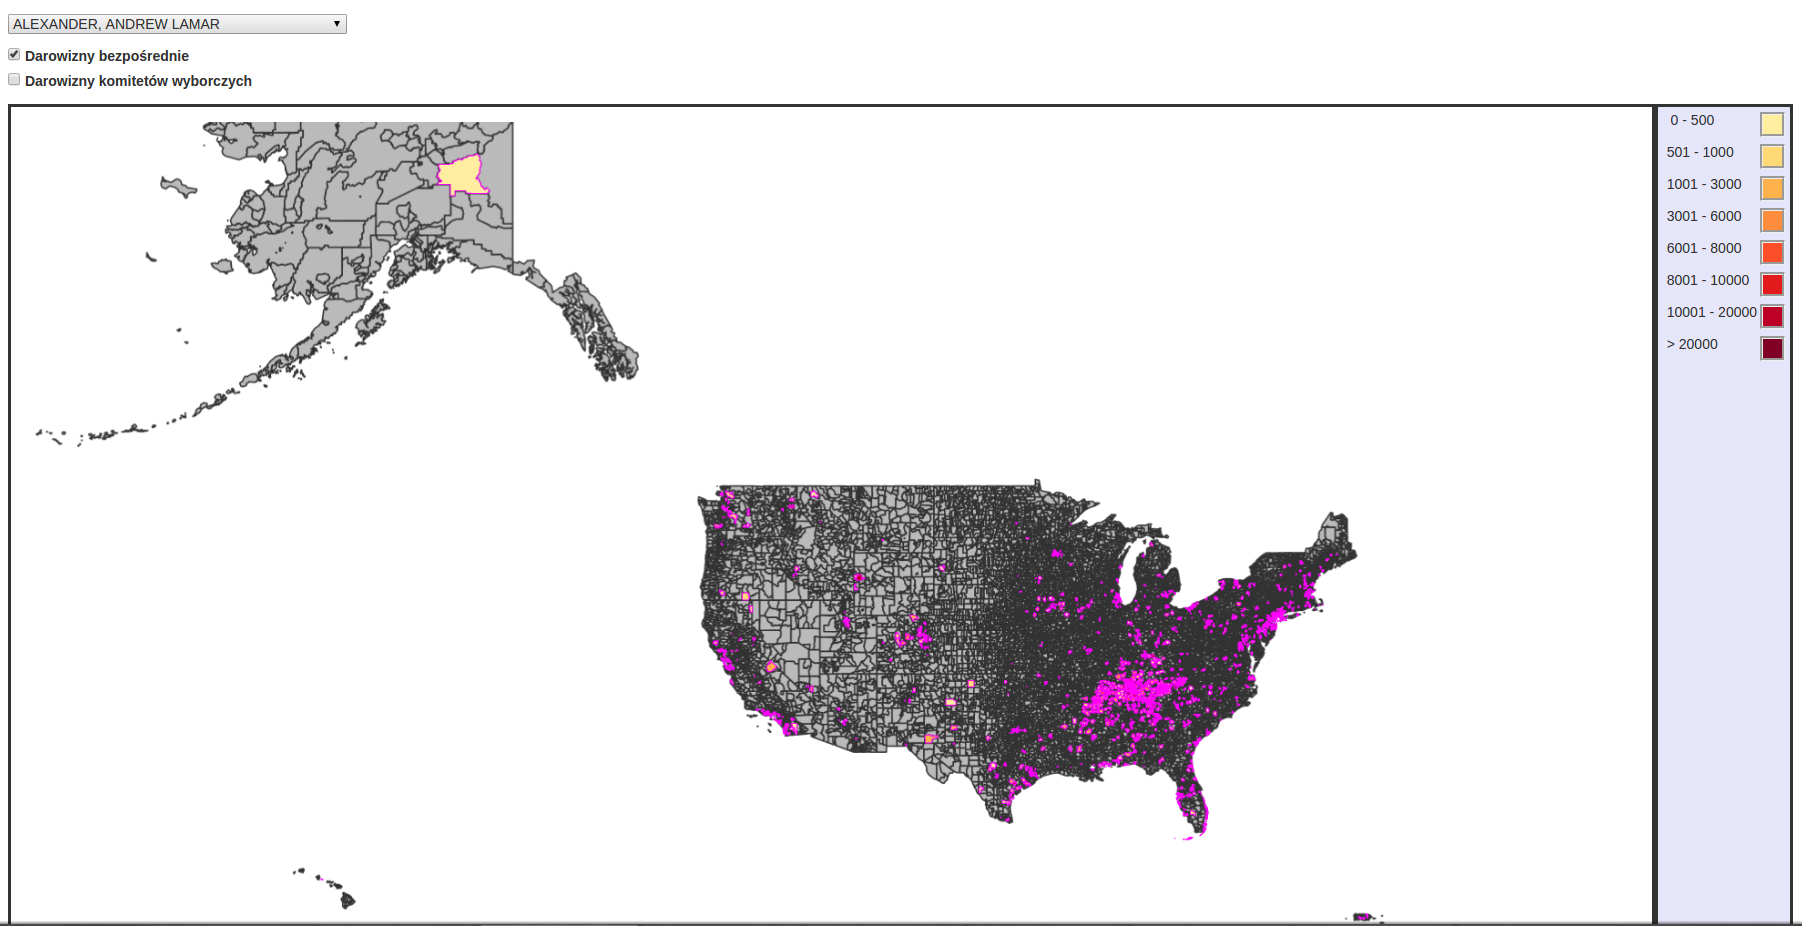
\includegraphics[width=1.0\textwidth]{whole.png}
    \caption{Całe Stany Zjednoczone, mała skala mapy.}
\end{figure}
\begin{figure}[H]
    \centering
    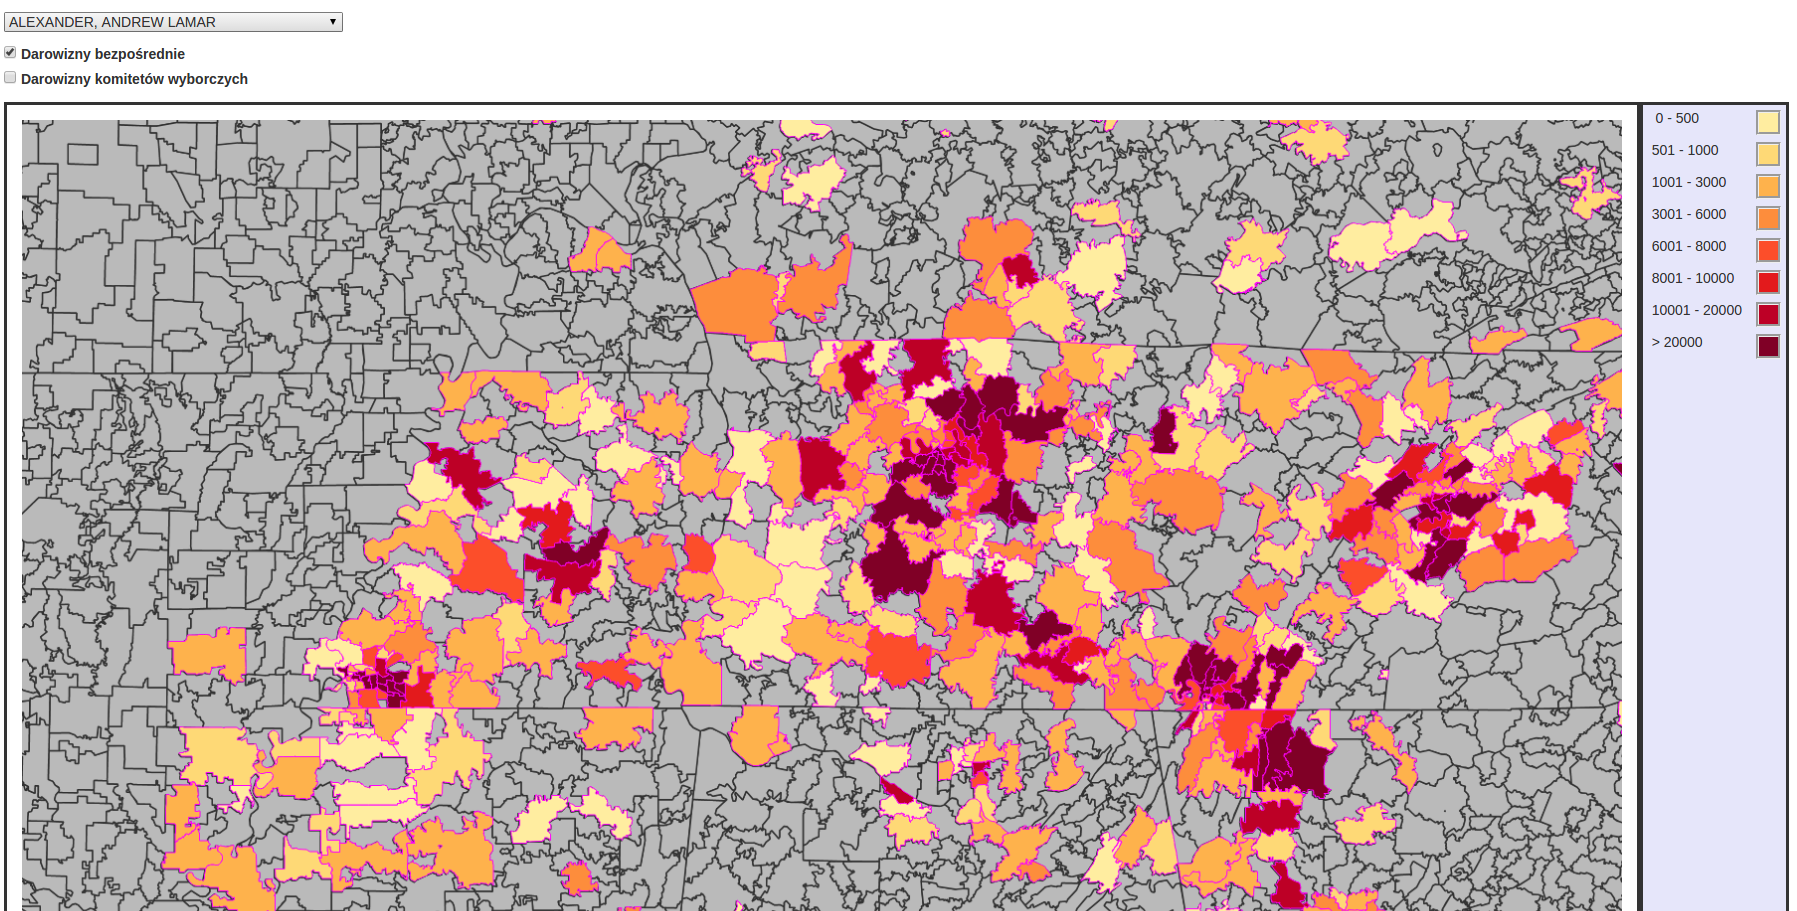
\includegraphics[width=1\textwidth]{medium.png}
    \caption{Średnia skala mapy.}
\end{figure}
\begin{figure}[H]
    \centering
    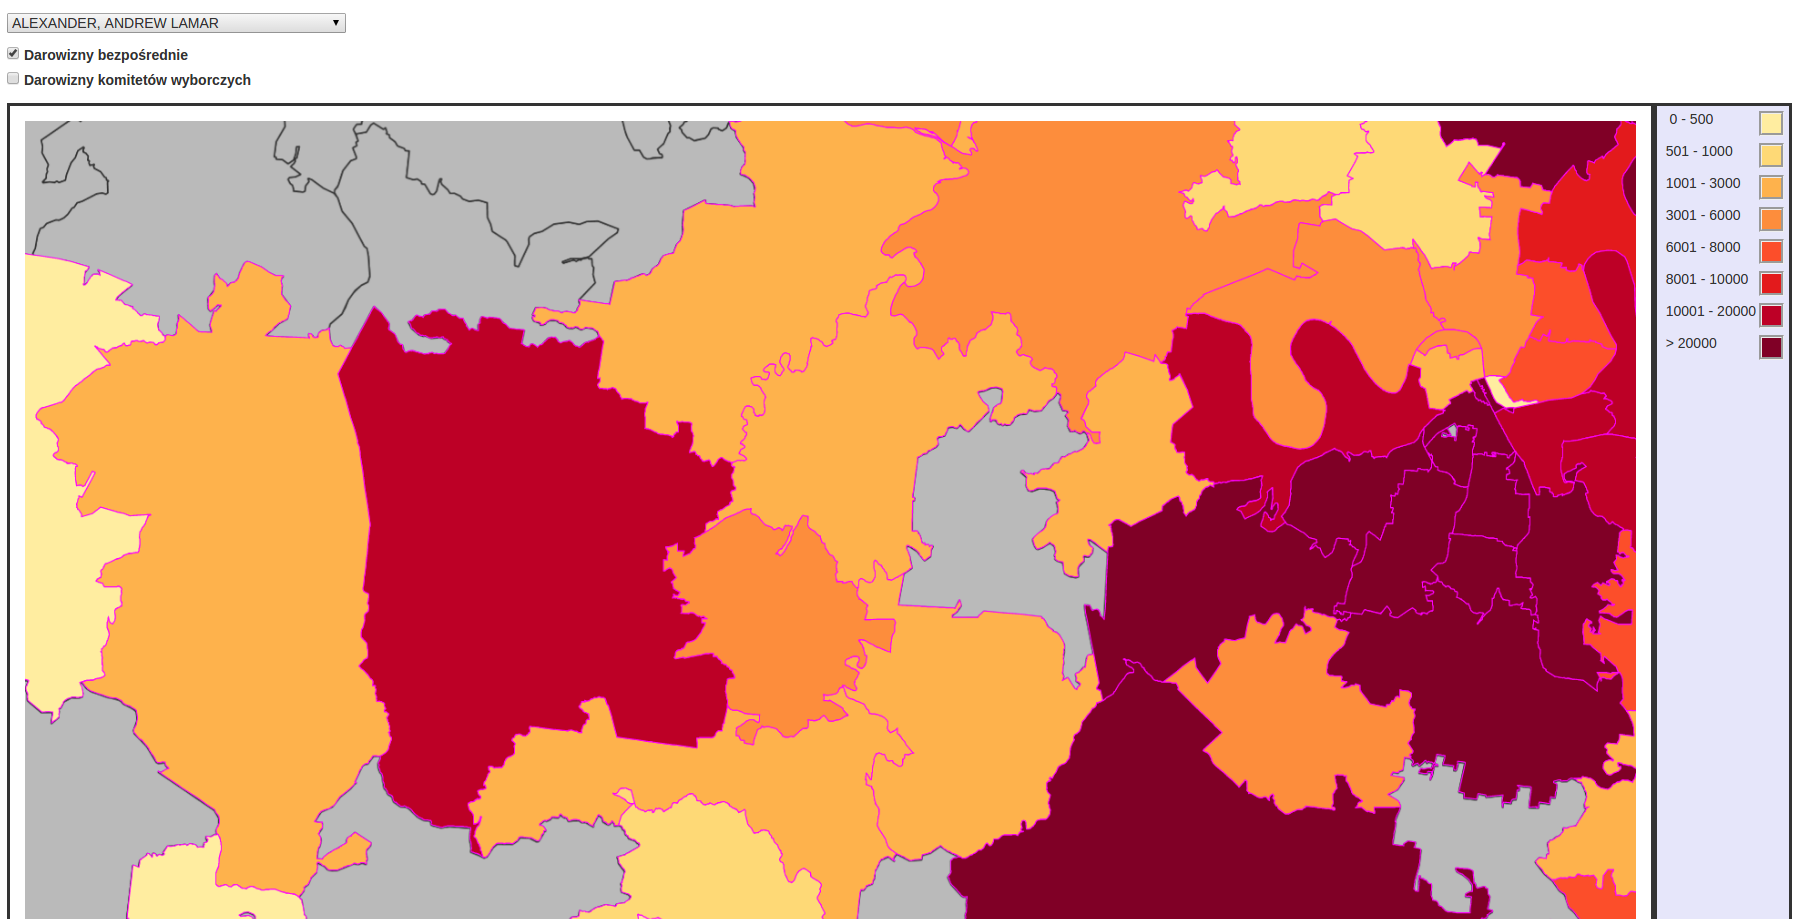
\includegraphics[width=1\textwidth]{small.png}
    \caption{Duża skala mapy.}
\end{figure}
\begin{figure}[H]
    \centering
    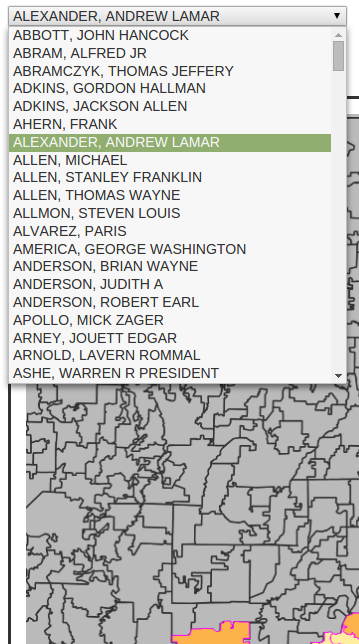
\includegraphics[width=0.4\textwidth]{selector.png}
    \caption{Wybór kandydata.}
\end{figure}

Jak widać na podstawie zrzutów niestety nie udało się nam w wyznaczonym czasie zrealizować agregacji danych w przypadku prezentacji danych na mapie o małej skali. Biblioteka openlayers udostępnia funkcjonalność \textit{clusteringu}, tak aby dało się grupować obiekty o odpowiednich wartościach. Inną możliwością mogłoby być zgrupowania konkretnych wartości dla danego stanu.

W stosunku do pierwotnej koncepcji nie zostało zrealizowane wybranie rocznika wyborów ze względu na duże ilości danych przechowywane w bazie danych byłoby niezwykle niewydajne trzymanie wszystkich danych w jednej tabeli, tak jak zrobiliśmy od początku. Chcąc dokonywać zapytań do tak dużych ilości danych należałoby się zastanowić nad lepszą organizacją danych w bazie danych.

\section{Załączniki}
Załączone archiwum składa się z następujących plików:
\begin{itemize}
\item[--] folder \textit{config} przechowujący konfigurację projektu,
\item[--] folder \textit{data-downloader} zawiera skrypty gradle umożliwiające pobranie danych oraz wykonanie skryptu tworzącego bazę danych (\textit{data-downloader/tass.sql}),
\item[--] folder \textit{data-db-extractor} zawierający skryptu w języku python umożliwiające napełnianie bazy danych pobranymi danymi,
\item[--] folder \textit{web-app} zawierający aplikację internetową.
\end{itemize}

Nie załączamy w przesłanym archiwum warstw SHP zawierających mapę Stanów Zjednoczony, ponieważ zajmuje ona 1.9 GB, jeśli zajdzie taka potrzeba możemy oczywiście dane nagrać na płytę bądź pendrive.

\bigskip

Poniżej zamieszczony został skrypt SQL tworzący strukturę bazy danych:
\begin{lstlisting}[style=BashInputStyle]
DROP RULE IF EXISTS 
"CANDIDATES_on_duplicate_ignore" ON CANDIDATES;
DROP RULE IF EXISTS
 "COMMITTEES_on_duplicate_ignore" ON COMMITTEES;
DROP RULE IF EXISTS
 "IND_CONTRIBS_on_duplicate_ignore" ON IND_CONTRIBS;
DROP RULE IF EXISTS
 "COMM_CONTRIBS_on_duplicate_ignore" ON COMM_CONTRIBS;
DROP RULE IF EXISTS
 "COMM_CAND_LINKAGES_on_duplicate_ignore" ON COMM_CAND_LINKAGES;

DROP TABLE IF EXISTS COMM_CAND_LINKAGES;
DROP TABLE IF EXISTS COMM_CONTRIBS;
DROP TABLE IF EXISTS IND_CONTRIBS;
DROP TABLE IF EXISTS COMMITTEES;
DROP TABLE IF EXISTS CANDIDATES;

CREATE TABLE CANDIDATES(
    CAND_ID VARCHAR(9) PRIMARY KEY,
    CAND_NAME VARCHAR(200),
    CAND_ELECTION_YR NUMERIC(4),
    CAND_CITY VARCHAR(30),
    CAND_ST VARCHAR(2),
    CAND_ZIP VARCHAR(9),
    CAND_OFFICE_ST VARCHAR(2),
    CAND_OFFICE VARCHAR(1),
    CAND_OFFICE_DISTRICT VARCHAR(2),
    CAND_PTY_AFFILIATION VARCHAR(3)
);

CREATE TABLE COMMITTEES(
    CMTE_ID VARCHAR(9) PRIMARY KEY,
    CMTE_NM VARCHAR(200),
    CMTE_CITY VARCHAR(30),
    CMTE_ST VARCHAR(2),
    CMTE_ZIP VARCHAR(9),
    CAND_ID VARCHAR(9),
    CMTE_TP VARCHAR(1),
    CMTE_PTY_AFFILIATION VARCHAR(3),
    FOREIGN KEY (CAND_ID) REFERENCES CANDIDATES(CAND_ID)
);

CREATE TABLE COMM_CAND_LINKAGES(
    LINKAGE_ID VARCHAR(9) PRIMARY KEY,
    CAND_ID VARCHAR(9),
    CAND_ELECTION_YR NUMERIC(4),
    FEC_ELECTION_YR NUMERIC(4),
    CMTE_ID VARCHAR(9),
    CMTE_TP VARCHAR(1),
    CMTE_DSGN VARCHAR(1),
    FOREIGN KEY (CAND_ID) REFERENCES CANDIDATES (CAND_ID),
    FOREIGN KEY (CMTE_ID) REFERENCES COMMITTEES (CMTE_ID)
);

CREATE TABLE COMM_CONTRIBS(
    SUB_ID NUMERIC(19) PRIMARY KEY,
    CMTE_ID VARCHAR(9),
    ENTITY_TP VARCHAR(3),
    NAME VARCHAR(200),
    CITY VARCHAR(30),
    STATE VARCHAR(2),
    ZIP_CODE VARCHAR(9),
    CAND_ID VARCHAR(9),
    TRANSACTION_AMT NUMERIC(14,2),
    TRANSACTION_DT DATE,
    FOREIGN KEY (CAND_ID) REFERENCES CANDIDATES (CAND_ID),
    FOREIGN KEY (CMTE_ID) REFERENCES COMMITTEES (CMTE_ID)
);

CREATE TABLE IND_CONTRIBS(
    SUB_ID NUMBER(19) PRIMARY KEY,
    CMTE_ID VARCHAR(9),
    ENTITY_TP VARCHAR(3),
    NAME VARCHAR(200),
    CITY VARCHAR(30),
    STATE VARCHAR(2),
    ZIP_CODE VARCHAR(9),
    TRANSACTION_AMT NUMERIC(14,2),
    TRANSACTION_DT DATE,
    FOREIGN KEY (CMTE_ID) REFERENCES COMMITTEES (CMTE_ID)
);

CREATE INDEX ON COMMITTEES (CMTE_ZIP);
CREATE INDEX ON COMMITTEES (CAND_ID);

CREATE INDEX ON CANDIDATES (CAND_ELECTION_YR);
CREATE INDEX ON CANDIDATES (CAND_ZIP);

CREATE INDEX ON COMM_CAND_LINKAGES (CAND_ELECTION_YR);
CREATE INDEX ON COMM_CAND_LINKAGES (CMTE_ID);

CREATE INDEX ON COMM_CONTRIBS (ZIP_CODE);
CREATE INDEX ON COMM_CONTRIBS (CAND_ID);
CREATE INDEX ON COMM_CONTRIBS (TRANSACTION_DT);
CREATE INDEX ON COMM_CONTRIBS (TRANSACTION_AMT);

CREATE INDEX ON IND_CONTRIBS (ZIP_CODE);
CREATE INDEX ON IND_CONTRIBS (TRANSACTION_DT);
CREATE INDEX ON IND_CONTRIBS (TRANSACTION_AMT);

CREATE RULE "CANDIDATES_on_duplicate_ignore" 
AS ON INSERT TO CANDIDATES
  WHERE EXISTS(SELECT 1 FROM CANDIDATES
                WHERE (CAND_ID)=(NEW.CAND_ID))
  DO INSTEAD NOTHING;

CREATE RULE "COMMITTEES_on_duplicate_ignore"
 AS ON INSERT TO COMMITTEES
  WHERE EXISTS(SELECT 1 FROM COMMITTEES
              WHERE (CMTE_ID)=(NEW.CMTE_ID))
  DO INSTEAD NOTHING;

CREATE RULE "IND_CONTRIBS_on_duplicate_ignore"
 AS ON INSERT TO IND_CONTRIBS
  WHERE EXISTS(SELECT 1 FROM IND_CONTRIBS
              WHERE (SUB_ID)=(NEW.SUB_ID))
  DO INSTEAD NOTHING;

CREATE RULE "COMM_CONTRIBS_on_duplicate_ignore"
 AS ON INSERT TO COMM_CONTRIBS
  WHERE EXISTS(SELECT 1 FROM COMM_CONTRIBS
              WHERE (SUB_ID)=(NEW.SUB_ID))
  DO INSTEAD NOTHING;

CREATE RULE "COMM_CAND_LINKAGES_on_duplicate_ignore" 
AS ON INSERT TO COMM_CAND_LINKAGES
  WHERE EXISTS(SELECT 1 FROM COMM_CAND_LINKAGES
              WHERE (LINKAGE_ID)=(NEW.LINKAGE_ID))
  DO INSTEAD NOTHING;

\end{lstlisting}

\end{document}